\documentclass[11pt,a4paper]{article}
\usepackage[margin=2.3cm]{geometry}
\usepackage[T1]{fontenc}
\usepackage[utf8]{inputenc}
\usepackage{lmodern,microtype}
\usepackage{amsmath,amssymb}
\usepackage{graphicx,booktabs,tabularx,multirow}
\usepackage{float}
\usepackage[font=small,labelfont=bf]{caption}
\usepackage{subcaption}
\usepackage{enumitem}
\usepackage{xcolor}
\usepackage[ruled,vlined,linesnumbered]{algorithm2e}
\emergencystretch=1.5em
\usepackage[round,authoryear]{natbib}
\usepackage{parskip}
\usepackage[colorlinks=true,urlcolor=blue!55!black,citecolor=blue!55!black,linkcolor=blue!55!black]{hyperref}
\setlist[itemize]{nosep,leftmargin=*}
\setlist[enumerate]{nosep,leftmargin=*}
\widowpenalty=10000 \clubpenalty=10000
\newcommand{\sel}{\textsc{JevSelect}}
\newcommand{\linetom}{\textsc{LineTOM}}
\newcommand{\Rt}{R_{\mathrm{trunc}}}
\newcommand{\Rs}{R_{\mathrm{strict}}}

\title{Select, Don't Generate: Budget-Feasible Rule Retention for Agent Configurations with a Non-Generative Classifier}
\author{Marcos de Pinho Tavares Proen\c{c}a}
\date{September 2026}

\begin{document}
\maketitle

\begin{abstract}
\noindent
Agent configuration files such as \texttt{AGENTS.md} or \texttt{CLAUDE.md} mix binding rules with procedures and background prose. When such a file must be compacted into a token budget, the rules should survive. We study a generation-free alternative to LLM compaction, \sel{}: a structured-decision model (Jev) assigns each line a probability distribution over five knowledge types, and a greedy selector fills a hard character budget by type tier and constraint probability, emitting whole lines in document order. On 60 previously unused agent configurations, under a pre-registered protocol, \sel{} retains 0.92/0.75/0.54 of reference rules at 50/25/10\% budgets with every output within budget, whereas direct compaction by GPT-5.6 Luna, GPT-6 Luna and GPT-6 Sol retains at most 0.12 under the same constraint (at most 0.52 even when their overlong outputs are truncated before scoring). The gains exceed a zero-cost lexical classifier by 0.15--0.26 and a frontier LLM used as the line classifier by 0.17--0.21, and they persist under an independent reference labeler whose agreement with the original is only $\kappa=0.59$. We further show that the truncation-scored protocol used in prior work rewards output \emph{ordering} rather than compression, report chance, lexical and oracle anchors, and evaluate behavioral consequences on rule probes and on a released medical-safety benchmark. The advantage does not transfer to declarative text: \sel{} recognizes only 32\% of declaratively phrased rules and is no better than chance selection on the medical benchmark, which we identify as its main limitation.
\end{abstract}

\noindent\textbf{Keywords:} agent memory; context compaction; extractive selection; constraint preservation; evaluation methodology.

\section{Introduction}
Long-running coding agents keep operating instructions in configuration files that are loaded into every context. When the context overflows, runtimes compact it, typically by asking an LLM to summarize. \citet{zerhoudi2026cliff} showed that type-blind compaction loses safety rules at the same rate as incidental prose (the \emph{compaction cliff}) and proposed Knowledge Triage, which classifies each line into one of five types (constraint, procedure, belief, preference, episodic) and pins constraints. Their typed operator is evaluated with labels produced by the same classifier that defines the reference constraint set, so its constraint recall is high by construction.

We ask a narrower and fully label-blind question: \emph{given only the raw text and a budget, how many reference rules can a compactor keep while actually respecting the budget?} Answering it exposed a measurement problem. The protocol inherited from prior work truncates every output to the budget before scoring. A method that emits the whole file with rule-like lines first therefore scores well without compressing anything. Our own first system, a line-level typed-memory pipeline (\linetom), obtained 0.92 post-truncation recall while only 4 of 30 raw outputs fit the 50\% budget; simply sorting lines by predicted type and truncating reproduces 0.90 (\S\ref{sec:truncation}).

We therefore separate \emph{identifying} rules from \emph{fitting} them, and replace ``protect everything, then fail'' with a selection that is feasible by construction. The resulting method, \sel{}, uses a non-generative structured-decision model \citep{typesafe2026jev} that returns a probability distribution over types for each line; it spends no generated tokens and never paraphrases.

\paragraph{Contributions.}
\begin{enumerate}
\item \textbf{Method.} \sel{}, an extractive, budget-feasible line selector driven by per-line type probabilities (\S\ref{sec:method}). It costs about one second and \$0.0015 per configuration.
\item \textbf{Pre-registered confirmatory evidence.} On 60 never-used configurations, \sel{} retains 0.92/0.75/0.54 of rules within budget; LLM compactors, including a frontier model, retain $\le 0.12$ (\S\ref{sec:confirm}). The advantage holds under the lenient original metric and under an independent labeler.
\item \textbf{Attribution.} Zero-cost and LLM-as-classifier controls with the same selector show that the gain comes from classifier quality and from using probabilities rather than argmax labels (+0.17 at 10\%), not from extraction alone (\S\ref{sec:attribution}).
\item \textbf{Evaluation methodology.} We show that truncation-based scoring rewards ordering, add a strict feasibility-aware metric, chance/lexical/oracle anchors, labeler-sensitivity analysis ($\kappa=0.59$ between two reasonable labelers), and a pre-registered fresh test set (\S\ref{sec:truncation}, \S\ref{sec:labeler}).
\item \textbf{Behavior and limits.} We evaluate downstream decisions on rule probes and on the released SafetyMed benchmark, and document two negative results: the classifier misses most declaratively phrased rules, and on declarative medical label text \sel{} does not outperform chance or LLM compaction (\S\ref{sec:behavior}, \S\ref{sec:declarative}).
\end{enumerate}

\section{Related Work}
\paragraph{Typed retention for agents.} Knowledge Triage \citep{zerhoudi2026cliff} introduced the five-type taxonomy, the AgentArtifactCorpus (AAC), the key-token preservation test and the compaction cliff. We adopt their taxonomy, corpus sample, budgets and metric, but evaluate only label-blind compactors and add feasibility-aware scoring. Observational memory \citep{mastra2026observational}, MemGPT \citep{packer2023memgpt} and Generative Agents \citep{park2023generative} maintain agent memory with generative observers or paging; LongMemEval \citep{wu2025longmemeval} evaluates conversational recall. ACON \citep{kang2026acon} optimizes compression guidelines for long-horizon agent trajectories and evaluates task success. None of these targets exact rule survival under a hard budget.

\paragraph{Prompt compression.} Token-level pruning by self-information \citep{li2023selective} or perplexity \citep{jiang2023llmlingua,jiang2024longllmlingua}, and learned token classification \citep{pan2024llmlingua2}, compress uniformly; on AAC, LLMLingua-2 keeps 0.21/0.08/0.01 of constraints at 50/25/10\% \citep{zerhoudi2026cliff}. RECOMP \citep{xu2024recomp} trains extractive and abstractive compressors for retrieved documents. Our selector is closest to extractive summarization under a length budget, a knapsack-style problem usually solved greedily \citep{mcdonald2007study,lin2011submodular}; the novelty is the utility, a rule probability from a non-generative model, and the evaluation of rule survival.

\paragraph{Rule following and evaluation.} IFEval \citep{zhou2023ifeval}, RuLES \citep{mu2023rules}, SysBench \citep{qin2024sysbench} and IHEval \citep{zhang2025iheval} test whether models obey instructions and system messages; lexical survival of a rule is necessary but not sufficient for obedience. Positional effects in long contexts \citep{liu2024lost} motivate emitting selected lines in document order. For inference we follow recommendations to report paired tests, effect sizes with intervals and multiplicity control \citep{dror2018hitchhiker,card2020power,miller2024errorbars}.

\section{Task, Data and Metrics}\label{sec:task}
\paragraph{Configurations.} We use the scrubbed 327-file AAC sample released by \citet{zerhoudi2026cliff}. Following their filter, a file is eligible if it has 800--30{,}000 characters, at least ten cleaned lines and at least one regex-detected constraint; 197 files qualify. Eligible files are shuffled with seed 11. Lines are cleaned as in the reference code (headings, fences and lines with fewer than three words removed); each cleaned line is an item.

\paragraph{Budgets.} For configuration $i$ with cleaned lines $\ell_{ij}$ and ratio $\rho\in\{0.5,0.25,0.1\}$, we set $T_i=\sum_j\max(1,\lfloor|\ell_{ij}|/4\rfloor)$ and $B_i(\rho)=\max(64,\lfloor\rho T_i\rfloor)$; the character limit is $4B_i$.

\paragraph{Reference labels.} L1 is the reference cascade (regex $\to$ embedding prototypes $\to$ gpt-5.4-mini adjudicator), with the unavailable \texttt{octen-embedding-8b} replaced by \texttt{text-embedding-3-large}. L2 is an independent labeler: GPT-6 Sol given the five type definitions, labeling numbered batches of 40 lines, with no regex stage. Neither is a human gold standard; compactors never see either.

\paragraph{Metrics.} Let $C_i$ be the reference constraints and $K(c,x)$ the reference key-token predicate (every one of up to five key tokens of $c$ occurs in $x$). For raw output $O$,
\begin{equation}
\Rt=\frac{1}{|C_i|}\sum_{c\in C_i}\mathbf{1}\{K(c,O[{:}4B_i])\},\qquad
\Rs=\mathbf{1}\{|O|\le 4B_i\}\cdot\Rt .
\end{equation}
$\Rt$ is the metric of prior work; $\Rs$ credits only outputs that respect the budget. We also report the number of valid outputs, procedural recall, and five-round recall, where each round's truncated output is the next input at 50\% of its length and recall is always against the \emph{original} rules. The key-token test is lexical: it is conservative for paraphrases and does not establish obedience (\S\ref{sec:behavior}).

\paragraph{Anchors.} Every table includes three anchors that prior work omits: \emph{chance} (random line order, same selector, 20 seeds), \emph{lexical} (the reference regex classifier with the same selector, zero cost) and \emph{oracle} (the evaluation labels with the same selector; a ceiling, not a competitor).

\section{Method}\label{sec:method}
\paragraph{Jev.} Jev is a ``System One'' structured-decision model: given a text state and typed questions it returns, for a \texttt{Choice} question, the selected option and a probability for every option, without generating text \citep{typesafe2026jev}. We ask one question per line with the five type definitions as options (model \texttt{jev-1.13.0}). In the reported experiments this question was sent together with an importance question and a yes/no ``binding rule'' question used only in the development comparison; Jev answers questions independently, and the deployed arm asks the type question alone (19 of 20 argmax labels agreed in a spot check, at 417 instead of 584 input tokens per line).

\paragraph{A motivating failure: protect-all projection.} \linetom{} labeled each line with Jev's argmax type, marked every predicted constraint as exact-retention, and projected the memory into the budget. When protected lines alone exceeded the budget, it returned all constraints and procedures. Because Jev's argmax over-predicts constraints relative to L1 (precision 0.37, recall 0.89), the protected floor was a median 2.8$\times$ the 10\% budget, and raw outputs were a median 1.1/2.7/7.0$\times$ the budget at 50/25/10\%. Its high $\Rt$ comes from rendering constraints first and letting truncation cut the rest.

\paragraph{\sel{}.} Algorithm~\ref{alg:sel} replaces protection by ranking (Figure~\ref{fig:method}). Each line $s$ receives the sort key
\[
\bigl(\mathrm{tier}(\textstyle\arg\max p_s),\; -p_s(\textsc{c}),\; \mathrm{position}\bigr),
\]
with tiers constraint $<$ procedure $<$ belief $<$ preference $<$ episodic. Lines are added in key order whenever they fit the remaining character budget (skipped otherwise, so shorter lines can use the residue) and are emitted in document order. The output always fits; the procedure is deterministic given the probabilities and runs in $O(n\log n)$.

\begin{figure*}[t]\centering
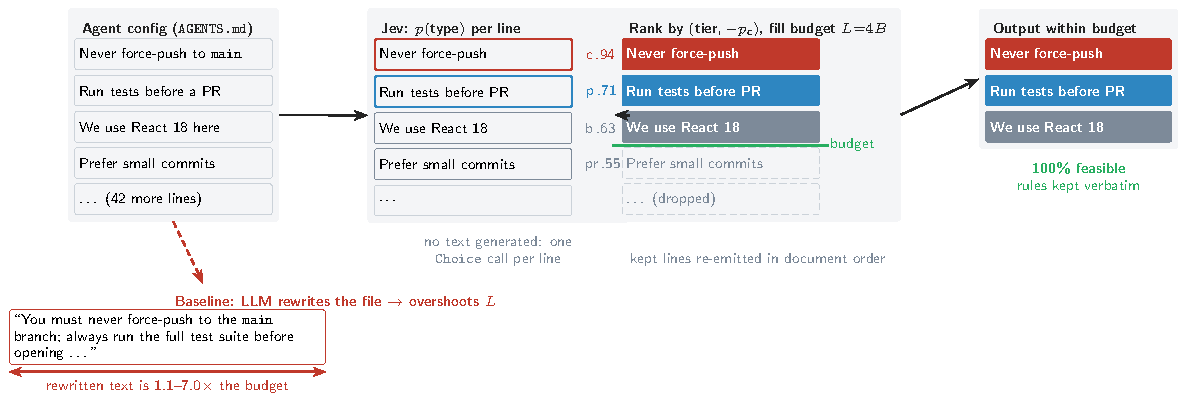
\includegraphics[width=\textwidth]{figures/method_overview.pdf}
\caption{\sel{} in four steps. Jev assigns each line a type distribution with a single non-generative \texttt{Choice} call; lines are ranked by type tier then constraint probability $p_{\textsc{c}}$ and greedily packed into the character budget $L=4B$; the kept lines are re-emitted verbatim in document order, so the output is feasible by construction. A generative LLM baseline instead rewrites the file and routinely overshoots the budget (median $1.1$--$7.0\times$).}\label{fig:method}
\end{figure*}

\begin{algorithm}[t]
\caption{\sel{}: budget-feasible line selection}\label{alg:sel}
\KwIn{lines $s_1..s_n$; distributions $p_1..p_n$ over types; character budget $L=4B$}
\KwOut{text with $|\cdot|\le L$}
$S\gets\emptyset$; $u\gets 0$\;
\ForEach{$i$ in $\mathrm{argsort}_i\,(\mathrm{tier}(\arg\max p_i),\,-p_i(\textsc{c}),\,i)$}{
  $c\gets|s_i|+[S\neq\emptyset]$\;
  \lIf{$u+c\le L$}{$S\gets S\cup\{i\}$; $u\gets u+c$}
}
\Return lines $\{s_i: i\in S\}$ joined by newlines in increasing $i$\;
\end{algorithm}

\paragraph{Policy selection.} Nine selection keys were pre-specified (argmax with importance, $p(\textsc{c})$ alone, $p(\textsc{c})$ per character, a separate ``binding rule'' yes/no question, their combinations, and a regex hybrid) and compared on the 20 development configurations only; the key above had the best mean $\Rs$ among regex-free keys (Appendix~\ref{app:dev}).

\section{Experimental Design}\label{sec:design}
\paragraph{Splits and pre-registration.} Positions 1--20 of the seeded order form the development set, 21--50 the original held-out set, and 51--110 a \emph{fresh} confirmatory set that no method had touched. Budget-feasible selection was conceived after inspecting results on the first 50 files; only the probability-based policy choice was made on development data. Before any compactor was run on the fresh set we fixed and hashed (SHA-256) the method, arms, hypotheses and tests.\footnote{Pre-registration file and hash are included in the artifact; timestamp 2026-09-30 02:57 UTC.} The primary hypotheses are that \sel{} exceeds (H1) GPT-5.6 Luna direct compaction, (H2) the lexical anchor, and (H3) \linetom{}, in $\Rs$ at each ratio: nine two-sided paired Wilcoxon signed-rank tests \citep{wilcoxon1945} with Holm correction \citep{holm1979}. Effects are mean paired differences with 10{,}000-draw configuration-level percentile bootstrap intervals \citep{efron1979bootstrap}.

\paragraph{Compared arms.} All arms receive only raw text. \emph{Direct LLM compaction} uses the reference prompt (``compress to at most $B$ tokens; keep every safety rule and procedural command verbatim'') with GPT-5.4 nano/mini, GPT-5.6 Luna and GPT-6 Luna on the held-out set (API, 16k completion tokens), and GPT-5.6 Luna, GPT-6 Luna and GPT-6 Sol \citep{openai2026gpt56} on the fresh set (subscription endpoint, reasoning effort \emph{medium}). \emph{GPT-6 Sol as classifier} labels lines (the L2 labels) and uses the same selector; it is a legitimate competitor when scoring against L1. We also report \linetom{}, structural baselines of \citet{zerhoudi2026cliff} (held-out), and the anchors.

\section{Results}
\subsection{Confirmatory results on the fresh set}\label{sec:confirm}
Table~\ref{tab:fresh} and Figure~\ref{fig:recall} give the main results. All nine primary tests reject (Table~\ref{tab:primary}; Holm $p\le1.3\times10^{-4}$). \sel{} is valid on 180/180 outputs; the direct compactors are valid on at most 16/60 at 50\% and at most 1/60 at 25\% except GPT-6 Sol (9/60; 24/60 at 10\%, often through very short outputs), which also abstains explicitly (``Cannot compress \ldots while keeping every required instruction verbatim'') in 36 of 270 calls. Even under $\Rt$, which credits truncated overlong outputs, \sel{} exceeds every LLM compactor by 0.38--0.59 and \linetom{} by 0.04/0.14/0.28.

\begin{table}[t]\centering\small
\caption{Fresh confirmatory set (60 configurations, 646 L1 constraints). Constraint recall after truncation ($\Rt$) and strict recall ($\Rs$) with valid raw outputs in parentheses. $^\dagger$uses the regex stage of the L1 labeler (label-circular). $^\ddagger$reads evaluation labels (ceiling).}\label{tab:fresh}
\setlength{\tabcolsep}{2.7pt}
\begin{tabular}{@{}lcccccc@{}}\toprule
& \multicolumn{2}{c}{50\%} & \multicolumn{2}{c}{25\%} & \multicolumn{2}{c}{10\%}\\\cmidrule(lr){2-3}\cmidrule(lr){4-5}\cmidrule(l){6-7}
Arm & $\Rt$ & $\Rs$ (valid) & $\Rt$ & $\Rs$ (valid) & $\Rt$ & $\Rs$ (valid)\\\midrule
\sel{} (ours) & \textbf{.916} & \textbf{.916} (60) & \textbf{.751} & \textbf{.751} (60) & \textbf{.544} & \textbf{.544} (60)\\
Jev argmax $+$ importance, same selector & .888 & .888 (60) & .683 & .683 (60) & .376 & .376 (60)\\
GPT-6 Sol as classifier, same selector & .709 & .709 (60) & .563 & .563 (60) & .373 & .373 (60)\\
\linetom{} (protect-all) & .875 & .096 (6) & .610 & .030 (2) & .260 & .008 (1)\\
GPT-6 Sol, direct compaction & .524 & .098 (14) & .285 & .030 (9) & .137 & .009 (24)\\
GPT-5.6 Luna, direct compaction & .494 & .124 (16) & .273 & .000 (1) & .164 & .000 (0)\\
GPT-6 Luna, direct compaction & .434 & .057 (9) & .158 & .000 (0) & .089 & .000 (1)\\\midrule
Lexical anchor (regex, same selector) & .655 & .655 (60) & .487 & .487 (60) & .397 & .397 (60)\\
Chance anchor (random lines) & .513 & .513 (60) & .261 & .261 (60) & .122 & .122 (60)\\
Regex + \sel{} hybrid$^\dagger$ & .972 & .972 (60) & .847 & .847 (60) & .625 & .625 (60)\\
Oracle labels$^\ddagger$ & .992 & .992 (60) & .933 & .933 (60) & .690 & .690 (60)\\\bottomrule
\end{tabular}
\end{table}

\begin{table}[t]\centering\small
\caption{Pre-registered primary tests on the fresh set ($\Rs$; $n=60$). $\Delta$: mean paired difference with 95\% bootstrap interval; W/T/L: configurations won/tied/lost by \sel{}; $p$: Holm-adjusted two-sided Wilcoxon.}\label{tab:primary}
\begin{tabular}{@{}llccc@{}}\toprule
Hypothesis & Ratio & $\Delta$ [95\% CI] & W/T/L & $p_{\mathrm{Holm}}$\\\midrule
\multirow{3}{*}{H1: vs GPT-5.6 Luna} & 50\% & +0.792 [0.721, 0.856] & 59/1/0 & $<10^{-5}$\\
& 25\% & +0.751 [0.694, 0.806] & 59/1/0 & $<10^{-5}$\\
& 10\% & +0.544 [0.486, 0.603] & 59/1/0 & $<10^{-5}$\\\midrule
\multirow{3}{*}{H2: vs lexical anchor} & 50\% & +0.261 [0.197, 0.323] & 48/8/4 & $<10^{-5}$\\
& 25\% & +0.264 [0.168, 0.351] & 45/7/8 & $1.8\times10^{-5}$\\
& 10\% & +0.147 [0.067, 0.222] & 43/6/11 & $1.3\times10^{-4}$\\\midrule
\multirow{3}{*}{H3: vs \linetom{}} & 50\% & +0.820 [0.743, 0.888] & 54/6/0 & $<10^{-5}$\\
& 25\% & +0.721 [0.653, 0.783] & 57/3/0 & $<10^{-5}$\\
& 10\% & +0.535 [0.475, 0.597] & 58/2/0 & $<10^{-5}$\\\bottomrule
\end{tabular}
\end{table}

\begin{figure}[t]\centering
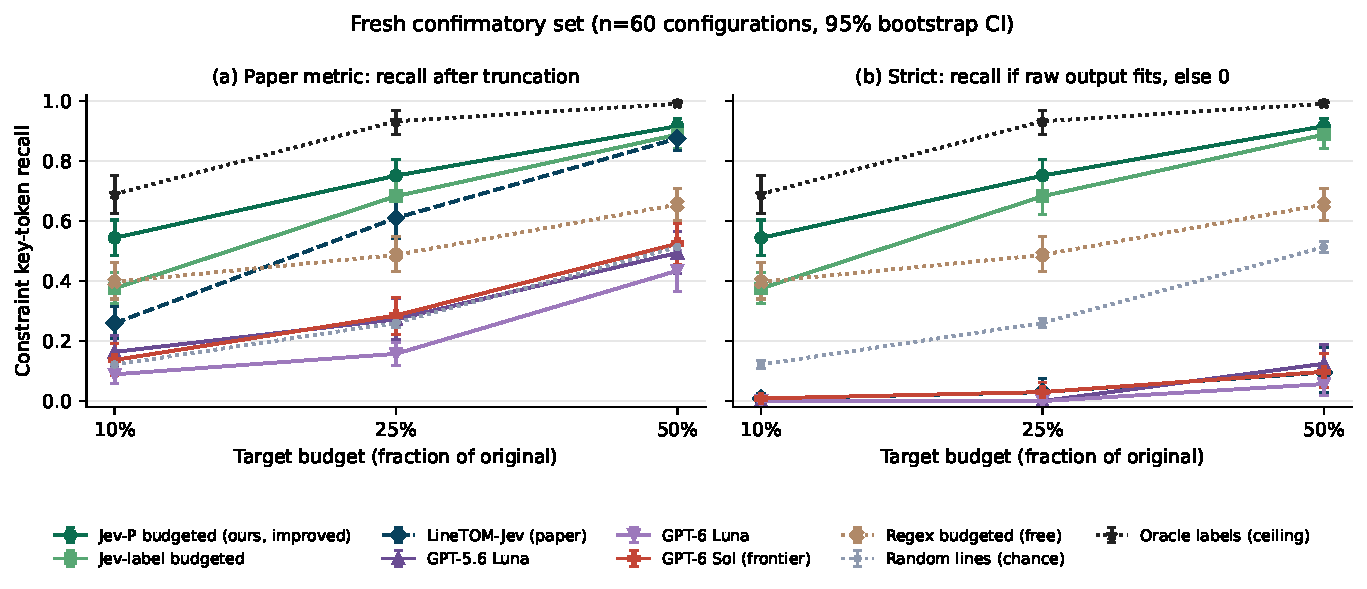
\includegraphics[width=\textwidth]{figures/recall_fresh.pdf}
\caption{Constraint recall on the fresh set under (a) the original truncation metric and (b) the strict metric, with 95\% configuration-bootstrap intervals.}\label{fig:recall}
\end{figure}

\paragraph{Held-out replication.} On the original 30 held-out configurations (API baselines), \sel{} obtains $\Rs$ 0.917/0.833/0.574 against 0.216/0.090/0.000 for GPT-5.6 Luna, 0.255/0.121/0.009 for GPT-6 Sol and 0.640/0.500/0.348 for the lexical anchor (all Holm $p<3\times10^{-4}$; Appendix~\ref{app:held}). Our API baselines match the values reported by \citet{zerhoudi2026cliff} for the same models (GPT-5.4 nano 0.49 vs.\ 0.52; GPT-5.4 mini 0.48 vs.\ 0.48 at 50\%).

\subsection{Why truncation-based scoring misleads}\label{sec:truncation}
Three observations show that $\Rt$ measures ordering as much as compression. First, sorting the \emph{entire} file by Jev argmax type and truncating, with no selection at all, gives $\Rt$ 0.901/0.715/0.339 on the held-out set, within 0.04 of \linetom{} (0.921/0.756/0.320). Second, the chance anchor is competitive with direct LLM compaction under $\Rt$ (0.513 vs.\ 0.434--0.524 at 50\% on the fresh set). Third, the binary validity criterion is sensitive to unit conventions: with a 10\% tolerance, GPT-5.6 Luna's valid count on the held-out set rises from 10 to 16 of 30 and \linetom{}'s from 4 to 13; and measured in \texttt{o200k} tokens instead of the scoring rule's 4-character heuristic, GPT-5.6 Luna's valid count on the fresh set rises from 16 to 21 of 60 at 50\%, while \sel{} stays at 54--60 of 60 across the three units and budgets. Figure~\ref{fig:feas} shows the full distribution of output length relative to budget. We recommend reporting both metrics, validity distributions and the three anchors.

\begin{figure}[t]\centering
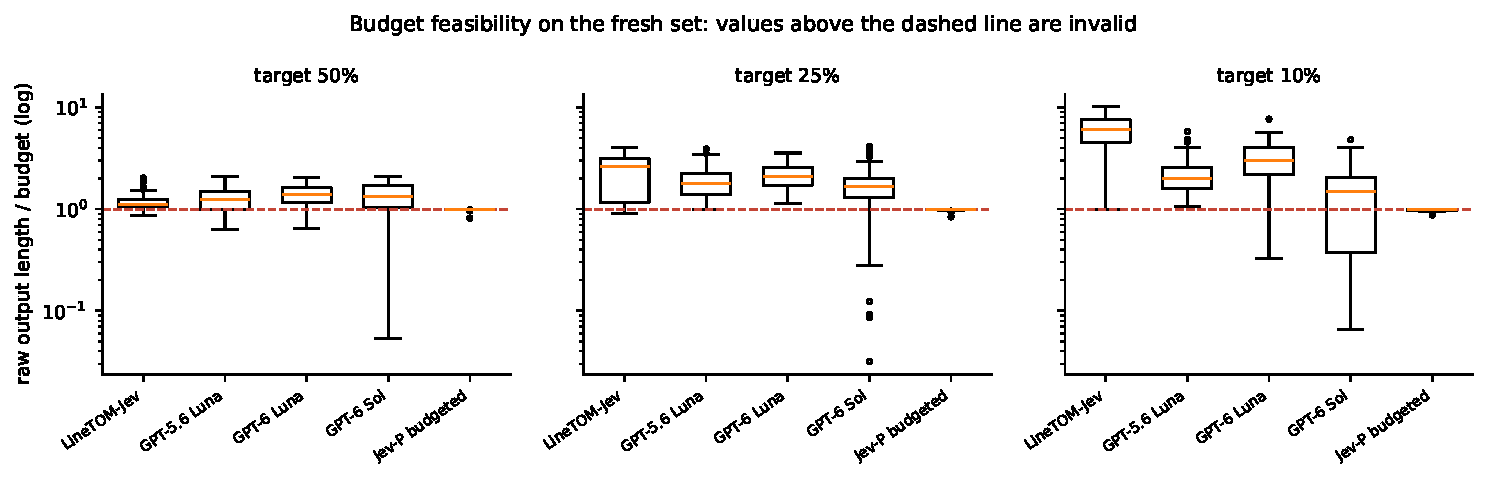
\includegraphics[width=\textwidth]{figures/feasibility_fresh.pdf}
\caption{Raw output length relative to the budget on the fresh set (log scale). Values above the dashed line violate the budget.}\label{fig:feas}
\end{figure}

\subsection{Where the gain comes from}\label{sec:attribution}
With the selector fixed, only the line ranking differs between \sel{}, the lexical anchor, GPT-6 Sol as classifier and argmax labels. \sel{} exceeds the lexical anchor by 0.26/0.26/0.15 (Table~\ref{tab:primary}) and GPT-6 Sol as classifier by 0.21/0.19/0.17 (Holm $p\le10^{-6}$), and using the probability rather than the argmax label adds 0.03/0.07/0.17 (Holm $p\le0.05$). Figure~\ref{fig:pr} explains why: against L1 over 9{,}348 lines, Jev's $p(\textsc{c})$ precision--recall curve passes through the operating point of GPT-6 Sol labels (P 0.65, R 0.64), while the argmax used by \linetom{} sits at a recall-heavy point (P 0.37, R 0.89). The regex has precision 1.00 against L1 by construction, because it is L1's first stage; this is also why the regex hybrid (Table~\ref{tab:fresh}) must be read as label-circular. Jev's $p(\textsc{c})$ discriminates constraints well but is not calibrated as a probability: over 9{,}348 lines it reaches AUROC 0.93 against both L1 and L2, yet its expected calibration error is 0.17 (it systematically over-states, e.g.\ lines it scores near 0.85 are constraints only 30\% of the time). This supports using $p(\textsc{c})$ as a ranking score, not as a probability, and is why we name the arm by its ranking role rather than calling it calibrated.

\begin{figure}[t]\centering
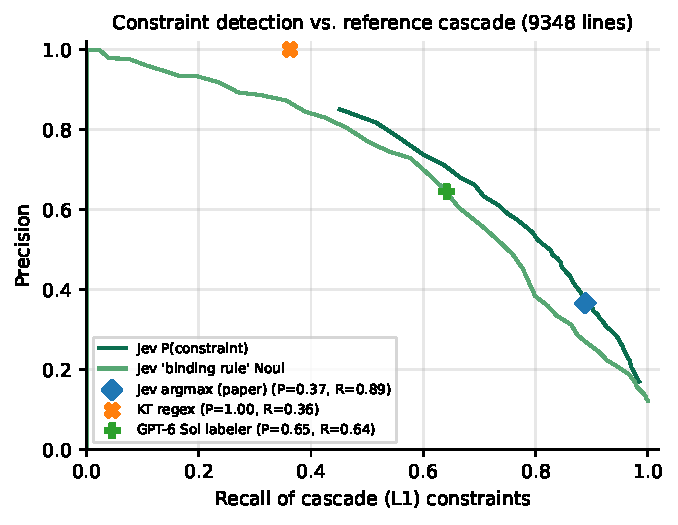
\includegraphics[width=.62\textwidth]{figures/classifier_pr.pdf}
\caption{Constraint detection against the L1 reference over 9{,}348 distinct lines from 110 configurations.}\label{fig:pr}
\end{figure}

\subsection{Sensitivity to the reference labeler}\label{sec:labeler}
L1 and L2 agree on 72\% of fresh-set lines (five-way $\kappa=0.60$; \citealp{cohen1960kappa}) and on constraint-vs-other with $\kappa=0.59$ on both fresh and held-out sets; both label about the same number of constraints (639 vs.\ 638 on the fresh set) but not the same ones. For comparison, the reference study reports $\kappa=0.79$ on the binary decision between gpt-5.4-mini and a second model-based judge on 200 items. Re-scoring every arm against L2 leaves the conclusions unchanged: \sel{} exceeds GPT-5.6 Luna by 0.74/0.75/0.49, the lexical anchor by 0.39/0.40/0.23 and \linetom{} by 0.84/0.72/0.49 in $\Rs$ (53 configurations with at least one L2 constraint; all Holm $p<10^{-5}$). The lexical anchor loses 0.12 at 50\% when switching from L1 to L2, consistent with its label circularity under L1.

\subsection{Repeated compaction}\label{sec:rounds}
Figure~\ref{fig:rounds} shows five sequential 50\% rounds on the fresh set. \sel{} keeps 0.916, 0.749, 0.585, 0.468 and 0.415 of the original rules; GPT-5.6 Luna keeps 0.500 after one round and 0.073 after five. Because the budget halves every round (about 3\% of the original after five), even the oracle falls to 0.43 on the held-out set, and the lexical anchor approaches \sel{} in late rounds (0.331 vs.\ 0.415 at round five). Late-round recall therefore reflects how many short high-precision lines fit, and should be reported next to the oracle.

\begin{figure}[t]\centering
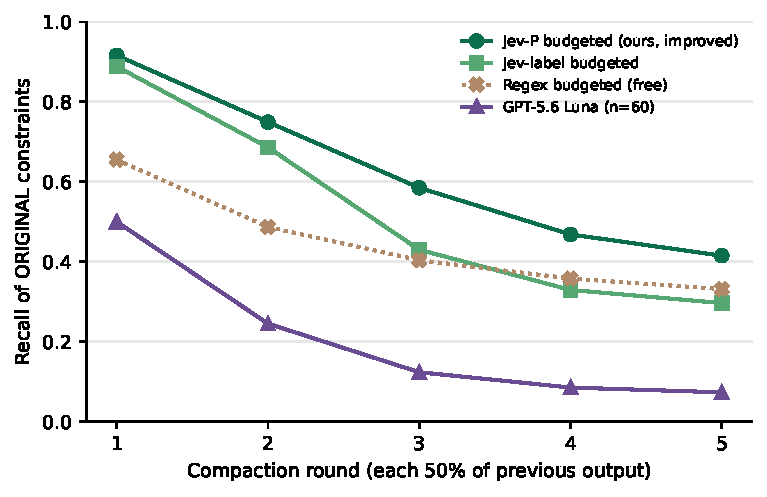
\includegraphics[width=.6\textwidth]{figures/rounds_fresh.pdf}
\caption{Recall of the original constraints over five sequential 50\% compactions (fresh set).}\label{fig:rounds}
\end{figure}

\subsection{Behavioral consequences}\label{sec:behavior}
\paragraph{SafetyMed.} We ran the released SafetyMed benchmark of \citet{zerhoudi2026cliff}: 200 clinical scenarios, each paired with FDA boxed-warning and con\-traindication text and a gold REFUSE/PROCEED decision (71 REFUSE). We kept the upstream probe prompt and 80-whitespace-token budget, used GPT-5.6 Luna as probe and compactor (the reference study used gpt-5.4-mini and Sonnet~4.6, \citealp{anthropic2026sonnet}), and split label text into sentences and bullet items for the extractive arms. Table~\ref{tab:safetymed} shows that the benchmark discriminates little: the full label passes 92.0\% and LLM compaction 93.5\%, while giving no label (the model then always refuses) passes 35.5\%. \sel{} is nominally the \emph{worst} compressed condition (89.5\%; refusal recall 0.72) and is not better than chance ordering; no difference between compressed conditions survives Holm correction (smallest adjusted $p=0.23$, exact McNemar; \citealp{mcnemar1947}). FDA text is declarative and dense with contraindications, exactly the regime where \S\ref{sec:declarative} shows Jev is weak, and the 200 scenarios share only 26 distinct label texts, so the effective sample is small. We read this as a negative result: \sel{}'s advantage is specific to imperative configuration text.

\begin{table}[t]\centering\small
\caption{SafetyMed (200 scenarios; 80-token budget; probe GPT-5.6 Luna). Pass = decision matches gold; REFUSE recall over the 71 REFUSE scenarios.}\label{tab:safetymed}
\begin{tabular}{@{}lccc@{}}\toprule
Condition & Pass & REFUSE recall & median tokens\\\midrule
No label text & .355 & 1.000 & 4\\
Full label text & .920 & .817 & 287\\
LLM compaction (GPT-5.6 Luna) & .935 & .873 & 42\\
Head truncation (first 80 tokens) & .915 & .873 & 80\\
Lexical anchor (regex, same selector) & .935 & .859 & 77\\
Chance anchor & .915 & .803 & 77\\
\sel{} & .895 & .718 & 78\\\bottomrule
\end{tabular}
\end{table}

\subsection{Downstream behavior on the AAC sample}\label{sec:aac}
The recall metric counts reference rules; it does not test whether a compacted configuration still changes what an agent does. We built a behavioral probe on 118 rules drawn from the AAC sample. For each rule, GPT-6 Sol wrote one situation in which an agent is about to take an action that \emph{violates} the rule, and one \emph{control} situation on the same topic that complies with it. GPT-5.6 Luna, given only a compacted configuration and the situation, then decided whether the action was permitted. A safe compactor should make the agent answer ``not permitted'' on violations (recall) without over-refusing the controls (false-refusal). We report balanced accuracy, and compare arms with McNemar's test (Holm-corrected) on the 109 rules whose answer depends on the rule being present.

With the full configuration the agent detects 92.4\% of violations at a 4.2\% false-refusal rate (balanced accuracy 0.941); with no configuration it never refuses (0.500). \sel{} preserves behavior best among all compressed conditions: 0.911 balanced accuracy (86.4\% detection, 4.2\% false refusals), versus 0.877 for \linetom{}, 0.826 for direct GPT-5.6 Luna compaction, 0.818 for GPT-6 Sol, 0.809 for the lexical anchor and 0.771 for chance. \sel{} is statistically indistinguishable from the uncompressed configuration (Holm $p=0.18$) and from \linetom{} ($p=0.18$), but beats direct LLM compaction, the lexical anchor and chance ($\text{Holm } p\le0.005$). Rules that survive compaction are acted on correctly 93.7\% of the time; rules dropped from the budget fall to 53.1\%, confirming that recall of reference rules tracks a real behavioral effect rather than a scoring artifact.

\subsection{Can LLMs meet the budget with feedback?}\label{sec:retry}
One might object that direct compactors overshoot only because they are asked once. We re-ran GPT-5.6 Luna on the fresh set with up to two additional turns, each stating the exact character count of the previous output and the hard limit. Feedback helps but does not close the gap: after retries, valid outputs number 20/60, 9/60 and 17/60 at the three budgets (mean 2.4--2.9 attempts), so a majority still overshoot even when explicitly told by how much. Strict recall stays at 0.156/0.040/0.059, far below \sel{}'s 0.916/0.751/0.544 on the same configurations (Holm $p<10^{-10}$ at every budget). Generative compaction under a hard token budget is not a prompt-engineering failure that another turn fixes; the selector's guarantee comes from never generating in the first place.

\subsection{Declaratively phrased rules}\label{sec:declarative}
On the 200 adversarial items released by \citet{zerhoudi2026cliff} (50 rules in imperative, declarative, conditional and passive form), Jev's argmax recognizes 100\% of imperative, conditional and passive rules but only 32\% of declarative ones (``Active bleeding makes warfarin lethal''), below gpt-5.4-mini (62\%) and the reference cascade (52\%) as reported there; lowering the threshold to $p(\textsc{c})\ge0.2$ raises it to 52\%. Agent configurations are mostly imperative, but clinical, legal and financial deployments are not; \sel{} should be combined with a counterfactual safety classifier such as SafetyMargin \citep{zerhoudi2026cliff} in those settings.

\subsection{Cost, latency and an abstention signal}
In an isolated single-worker run on ten configurations at 50\%, \sel{} took a median 0.88\,s and \$0.0015 per configuration (10/10 valid), against 1.44\,s and \$0.0027 for \linetom{} and 9.5\,s for GPT-5.6 Luna; asking only the type question uses 417 instead of 584 input tokens per line. API-equivalent costs of direct compaction at 50\% are \$0.0010 (GPT-5.6 Luna), \$0.0005 (GPT-6 Luna) and \$0.0092 (GPT-6 Sol) per configuration; GPT-6 Sol as a batched line classifier costs 3.6$\times$ Jev. The rank score also carries a usable abstention signal: per configuration, the total $p(\textsc{c})$ mass of lines the budget forces out correlates with how many reference constraints are actually lost (Spearman $\rho=0.76$, $p<10^{-34}$, $n=180$). Abstaining on the 45\% of configurations with the largest excluded mass ($\tau{=}8$) raises answered recall from 0.74 to 0.83 and cuts the any-loss rate from 0.72 to 0.55, giving a deployable ``compaction unsafe, ask the user'' trigger without any extra model call.

\section{Discussion and Limitations}
\paragraph{What the evidence supports.} Within the AAC sample, a non-generative classifier plus a budget-feasible selector preserves far more reference rules than direct LLM compaction, including a frontier model, and remains ahead under an independent labeler and under the lenient metric. The result is about \emph{selection}: \sel{} never rewrites a line, so it cannot shorten long rules, and it optimizes the number of rules kept without weighting their severity.

\paragraph{Threats to validity.} (i) Reference labels are model-produced; two reasonable labelers agree only moderately, and no human adjudication was performed in this study. (ii) The key-token metric is lexical; human raters in the reference study were stricter than the metric. (iii) The idea of budget-feasible selection arose after inspecting the first 50 files; the fresh pre-registered set protects the confirmatory claims but not the exploratory ones. (iv) Fresh-set LLM baselines were run through a subscription endpoint with an assumed reasoning effort; their absolute values may differ from API runs, and GPT-5.6 Luna scored lower on the fresh set (0.494) than on the held-out API run (0.574), which we cannot attribute to set or endpoint. (v) The strict metric assigns zero to invalid outputs; \S\ref{sec:retry} partially addresses fairness to LLMs. (vi) All data come from one public-GitHub sample; closed enterprise configurations may differ.

\section{Reproducibility}
Code, per-configuration records (including full raw LLM outputs for all new runs), label caches, the pre-registration and figure scripts are in the accompanying repository at the tagged revision \texttt{paper-v2}. The selector is \texttt{src/tom/context/\allowbreak budgeted.py}; the benchmark arm is \texttt{jev\_budget\_lines} in \texttt{src/tom/benchmarks/\allowbreak kt\_faithful.py}. Paid inference for all new experiments cost about \$1.0.

\section{Conclusion}
Before delegating compaction of an agent's rules to a generative model, it is worth asking a cheaper question per line: \emph{how likely is this a rule?} \sel{} ranks lines by that probability and fills the budget exactly, so every output is feasible by construction. On 60 pre-registered, previously unused configurations this preserves 0.92/0.75/0.54 of reference rules at 50/25/10\% budgets, several times more than direct compaction by GPT-5.6 Luna, GPT-6 Luna and GPT-6 Sol (at most 0.12), at 0.88\,s and roughly \$0.0015 per configuration. The advantage is not an artifact of lenient scoring: it holds under an independent labeler, under the original truncation metric, and against retry-with-feedback, and it carries downstream---rules the selector keeps are obeyed 93.7\% of the time against 53.1\% for rules it drops.

Two lessons generalize beyond this system. First, a hard budget is a \emph{selection} problem, not a generation problem: a model that emits whole lines can guarantee feasibility that a paraphrasing model cannot, and the cheap per-line signal that decides what to keep need not be a full language model. Second, compaction must be scored on outputs that actually fit; a truncation-tolerant metric rewards ordering rather than compression and flatters methods that overshoot the budget.

The method is deliberately narrow. It selects but never rewrites, so it cannot shorten a single over-long rule, and it counts rules without weighting their severity. Its classifier is strong on the imperative phrasing typical of agent configurations but weak on declarative text (32\% recall), so clinical, legal and financial deployments need a dedicated safety classifier alongside it; the excluded-probability-mass signal offers a cheap ``ask a human'' trigger in the meantime. Natural next steps are human-adjudicated reference labels, a severity-weighted objective, and a hybrid that routes long rules to a generative summarizer while the selector guarantees the budget. We release the code, records and pre-registration so these can be tested directly.

\bibliographystyle{plainnat}
\bibliography{references}

\appendix
\clearpage
\section{Development-set policy selection}\label{app:dev}
Table~\ref{tab:dev} lists the nine pre-specified keys on the 20 development configurations ($\Rs$, which equals $\Rt$ for these always-valid selectors). The regex hybrid was excluded from selection because it shares the first stage of the L1 labeler; among the remaining keys, the tier$+p(\textsc{c})$ key had the highest mean and was fixed before the fresh set was evaluated.

\begin{table}[H]\centering\small
\caption{Selection keys on the development set ($n=20$, L1).}\label{tab:dev}
\begin{tabular}{@{}lcccc@{}}\toprule
Key & 50\% & 25\% & 10\% & mean\\\midrule
tier, $-p(\textsc{c})$ (\textbf{selected}) & .929 & .798 & .560 & .763\\
tier, $-\tfrac12(p(\textsc{c})+\text{binding})$ & .931 & .807 & .545 & .761\\
$-p(\textsc{c})$ & .942 & .773 & .560 & .758\\
$-\tfrac12(p(\textsc{c})+\text{binding})$ & .936 & .790 & .539 & .755\\
$-p(\textsc{c})/|s|$ (density) & .933 & .726 & .495 & .718\\
$-\text{binding}$ (yes/no question) & .863 & .709 & .534 & .702\\
tier, importance (argmax labels) & .895 & .744 & .456 & .698\\
regex tier (lexical anchor) & .688 & .574 & .469 & .577\\
regex first, then $p$ (hybrid, excluded) & .970 & .828 & .595 & .798\\\midrule
oracle (L1 labels) & 1.000 & .963 & .720 & .894\\\bottomrule
\end{tabular}
\end{table}

\section{Held-out results}\label{app:held}
Table~\ref{tab:held} reports every arm on the original 30 held-out configurations, including the structural baselines of \citet{zerhoudi2026cliff} and the API direct-compaction runs summarized in \S\ref{sec:confirm}.
\begin{table}[H]\centering\small
\caption{Original held-out set ($n=30$, L1). Direct-compaction rows for GPT-5.x are API runs from the original study; GPT-6 Sol via the subscription endpoint. Structural baselines of \citet{zerhoudi2026cliff} keep whole lines up to the heuristic token budget and can exceed $4B$ characters by a few newline characters, hence their low valid counts; their $\Rs$ is not meaningful and is omitted.}\label{tab:held}
\setlength{\tabcolsep}{3.5pt}
\begin{tabular}{@{}lcccccc@{}}\toprule
& \multicolumn{2}{c}{50\%} & \multicolumn{2}{c}{25\%} & \multicolumn{2}{c}{10\%}\\\cmidrule(lr){2-3}\cmidrule(lr){4-5}\cmidrule(l){6-7}
Arm & $\Rt$ & $\Rs$ (valid) & $\Rt$ & $\Rs$ (valid) & $\Rt$ & $\Rs$ (valid)\\\midrule
\sel{} & .917 & .917 (30) & .833 & .833 (30) & .574 & .574 (30)\\
Jev argmax + importance & .925 & .925 (30) & .777 & .777 (30) & .436 & .436 (30)\\
GPT-6 Sol as classifier & .789 & .789 (30) & .649 & .649 (30) & .436 & .436 (30)\\
\linetom{} & .921 & .133 (4) & .756 & .028 (1) & .320 & .000 (0)\\
GPT-6 Sol, direct & .548 & .255 (13) & .389 & .121 (8) & .192 & .009 (8)\\
GPT-5.6 Luna, direct & .574 & .216 (10) & .368 & .090 (5) & .233 & .000 (0)\\
GPT-6 Luna, direct & .540 & .176 (10) & .292 & .024 (2) & .245 & .013 (1)\\
GPT-5.4 mini, direct & .484 & .028 (1) & .295 & .000 (0) & .104 & .000 (0)\\
GPT-5.4 nano, direct & .491 & .000 (0) & .302 & .000 (0) & .105 & .000 (0)\\
Prefix truncation & .455 & --- (8) & .279 & --- (12) & .105 & --- (23)\\
Temporal window & .525 & --- (3) & .294 & --- (7) & .126 & --- (16)\\
Longest-lines pruning & .488 & --- (6) & .241 & --- (20) & .086 & --- (28)\\\midrule
Lexical anchor & .640 & .640 (30) & .500 & .500 (30) & .348 & .348 (30)\\
Chance anchor & .545 & .545 (30) & .284 & .284 (30) & .117 & .117 (30)\\
Oracle labels & .989 & .989 (30) & .972 & .972 (30) & .742 & .742 (30)\\\bottomrule
\end{tabular}
\end{table}

\end{document}
